\documentclass[english]{article}
\newcommand{\G}{\overline{C_{2k-1}}}
\usepackage[latin9]{inputenc}
\usepackage{amsmath}
\usepackage{amssymb}
\usepackage{lmodern}
\usepackage{mathtools}
\usepackage{enumitem}

%\usepackage{natbib}
%\bibliographystyle{plainnat}
%\setcitestyle{authoryear,open={(},close={)}}
\let\avec=\vec
\renewcommand\vec{\mathbf}
\renewcommand{\d}[1]{\ensuremath{\operatorname{d}\!{#1}}}
\newcommand{\pydx}[2]{\frac{\partial #1}{\partial #2}}
\newcommand{\dydx}[2]{\frac{\d #1}{\d #2}}
\newcommand{\ddx}[1]{\frac{\d{}}{\d{#1}}}
\newcommand{\hk}{\hat{K}}
\newcommand{\hl}{\hat{\lambda}}
\newcommand{\ol}{\overline{\lambda}}
\newcommand{\om}{\overline{\mu}}
\newcommand{\all}{\text{all }}
\newcommand{\valph}{\vec{\alpha}}
\newcommand{\vbet}{\vec{\beta}}
\newcommand{\vT}{\vec{T}}
\newcommand{\vN}{\vec{N}}
\newcommand{\vB}{\vec{B}}
\newcommand{\vX}{\vec{X}}
\newcommand{\vx}{\vec {x}}
\newcommand{\vn}{\vec{n}}
\newcommand{\vxs}{\vec {x}^*}
\newcommand{\vV}{\vec{V}}
\newcommand{\vTa}{\vec{T}_\alpha}
\newcommand{\vNa}{\vec{N}_\alpha}
\newcommand{\vBa}{\vec{B}_\alpha}
\newcommand{\vTb}{\vec{T}_\beta}
\newcommand{\vNb}{\vec{N}_\beta}
\newcommand{\vBb}{\vec{B}_\beta}
\newcommand{\bvT}{\bar{\vT}}
\newcommand{\ka}{\kappa_\alpha}
\newcommand{\ta}{\tau_\alpha}
\newcommand{\kb}{\kappa_\beta}
\newcommand{\tb}{\tau_\beta}
\newcommand{\hth}{\hat{\theta}}
\newcommand{\evat}[3]{\left. #1\right|_{#2}^{#3}}
\newcommand{\prompt}[1]{\begin{prompt*}
		#1
\end{prompt*}}
\newcommand{\vy}{\vec{y}}
\DeclareMathOperator{\sech}{sech}
\DeclarePairedDelimiter\abs{\lvert}{\rvert}%
\DeclarePairedDelimiter\norm{\lVert}{\rVert}%
\newcommand{\dis}[1]{\begin{align*}
	#1
	\end{align*}}
\newcommand{\LL}{\mathcal{L}}
\newcommand{\RR}{\mathbb{R}}
\newcommand{\NN}{\mathbb{N}}
\newcommand{\ZZ}{\mathbb{Z}}
\newcommand{\QQ}{\mathbb{Q}}
\newcommand{\Ss}{\mathcal{S}}
\newcommand{\BB}{\mathcal{B}}
\newcommand{\ms}{\text{ m/s}}
\newcommand{\mss}{\text{ m/s}^2}
\newcommand{\ml}{\text{ m}}
\newcommand{\msa}{\text{ m}^2}
\newcommand{\st}{\text{ s}}
\newcommand{\rad}{\text{ rad}}
\newcommand{\rads}{\text{ rad/s}}
\newcommand{\radss}{\text{rad/s}^2}
\newcommand{\nf}{\text{ N}}
\newcommand{\kgm}{\text{ kg}}
\newcommand{\je}{\text{ J}}
\newcommand{\mje}{\text{ MJ}}
\newcommand{\kje}{\text{ kJ}}
\newcommand{\Wp}{\text{ W}}
\newcommand{\Wpms}{\text{ W/m}^2}
\newcommand{\kWp}{\text{ kW}}
\newcommand{\kWpms}{\text{ kW/m}^2}
\newcommand{\kgmt}{\kgm/\text{m}^3}
\newcommand{\nm}{\times 10^{-6}\ml}
\usepackage{graphicx}
% Swap the definition of \abs* and \norm*, so that \abs
% and \norm resizes the size of the brackets, and the 
% starred version does not.
%\makeatletter
%\let\oldabs\abs
%\def\abs{\@ifstar{\oldabs}{\oldabs*}}
%
%\let\oldnorm\norm
%\def\norm{\@ifstar{\oldnorm}{\oldnorm*}}
%\makeatother
\newenvironment{subproof}[1][\proofname]{%
	\renewcommand{\qedsymbol}{$\blacksquare$}%
	\begin{proof}[#1]%
	}{%
	\end{proof}%
}

\usepackage{centernot}
\usepackage{dirtytalk}
\usepackage{calc}
\newcommand{\prob}[1]{\setcounter{section}{#1-1}\section{}}
\newcommand{\prt}[1]{\setcounter{subsection}{#1-1}\subsection{}}
\newcommand{\pprt}[1]{{\textit{{#1}.)}}\newline}
\renewcommand\thesubsection{\alph{subsection}}
\usepackage[sl,bf,compact]{titlesec}
\titlelabel{\thetitle.)\quad}
\DeclarePairedDelimiter\floor{\lfloor}{\rfloor}
\makeatletter

\newcommand*\pFqskip{8mu}
\catcode`,\active
\newcommand*\pFq{\begingroup
	\catcode`\,\active
	\def ,{\mskip\pFqskip\relax}%
	\dopFq
}
\catcode`\,12
\def\dopFq#1#2#3#4#5{%
	{}_{#1}F_{#2}\biggl(\genfrac..{0pt}{}{#3}{#4}|#5\biggr
	)%
	\endgroup
}
\def\res{\mathop{Res}\limits}
% Symbols \wedge and \vee from mathabx
% \DeclareFontFamily{U}{matha}{\hyphenchar\font45}
% \DeclareFontShape{U}{matha}{m}{n}{
%       <5> <6> <7> <8> <9> <10> gen * matha
%       <10.95> matha10 <12> <14.4> <17.28> <20.74> <24.88> matha12
%       }{}
% \DeclareSymbolFont{matha}{U}{matha}{m}{n}
% \DeclareMathSymbol{\wedge}         {2}{matha}{"5E}
% \DeclareMathSymbol{\vee}           {2}{matha}{"5F}
% \makeatother

%\titlelabel{(\thesubsection)}
%\titlelabel{(\thesubsection)\quad}
\usepackage{listings}
\lstloadlanguages{[5.2]Mathematica}
\usepackage{babel}
\newcommand{\ffac}[2]{{(#1)}^{\underline{#2}}}
\usepackage{color}
\usepackage{amsthm}
\newtheorem{theorem}{Theorem}[section]
%\newtheorem*{theorem*}{Theorem}[section]
\newtheorem{conj}[theorem]{Conjecture}
\newtheorem{corollary}[theorem]{Corollary}
\newtheorem{example}[theorem]{Example}
\newtheorem{lemma}[theorem]{Lemma}
\newtheorem*{lemma*}{Lemma}
\newtheorem{problem}[theorem]{Problem}
\newtheorem{proposition}[theorem]{Proposition}
\newtheorem*{prop*}{Proposition}
\newtheorem*{corollary*}{Corollary}
\newtheorem{fact}[theorem]{Fact}

\newtheorem*{claim*}{Claim}
\newcommand{\claim}[1]{\begin{claim*} #1\end{claim*}}
%organizing theorem environments by style--by the way, should we really have definitions (and notations I guess) in proposition style? it makes SO much of our text italicized, which is weird.
\theoremstyle{remark}
\newtheorem{remark}{Remark}[section]

\theoremstyle{definition}
\newtheorem{definition}[theorem]{Definition}
\newtheorem{notation}[theorem]{Notation}
\newtheorem*{notation*}{Notation}

%FINAL
\newcommand{\due}{16 October 2017} 
\RequirePackage{geometry}
\geometry{margin=.7in}
\usepackage{todonotes}
\title{Worksheet for 10/16}
\author{David DeMark}
\date{\due}
\usepackage{fancyhdr}
\pagestyle{fancy}
\fancyhf{}
\rhead{Groups: \S3.7, 3.10, 4.1}
\chead{\due}
\lhead{MATH 1271-012\&016}
\cfoot{\thepage}
% %%
%%
%%
%DRAFT

%\usepackage[left=1cm,right=4.5cm,top=2cm,bottom=1.5cm,marginparwidth=4cm]{geometry}
%\usepackage{todonotes}
% \title{MATH 8669 Homework 4-DRAFT}
% \usepackage{fancyhdr}
% \pagestyle{fancy}
% \fancyhf{}
% \rhead{David DeMark}
% \lhead{MATH 8669-Homework 4-DRAFT}
% \cfoot{\thepage}

%PROBLEM SPEFICIC

\newcommand{\lint}{\underline{\int}}
\newcommand{\uint}{\overline{\int}}
\newcommand{\hfi}{\hat{f}^{-1}}
\newcommand{\tfi}{\tilde{f}^{-1}}
\newcommand{\tsi}{\tilde{f}^{-1}}
\newcommand{\PP}{\mathcal{P}}
\newcommand{\nin}{\centernot\in}
\newcommand{\seq}[1]{({#1}_n)_{n\geq 1}}
\usepackage{array}
\newcolumntype{M}[1]{>{\centering\arraybackslash}m{#1}}
\newcolumntype{N}{@{}m{0pt}@{}}
\input ArtNouvc.fd
\newcommand*\initfamily{\usefont{U}{ArtNouvc}{xl}{n}}
\begin{document}
%	\emph{\textbf{\large} As usual, take no more than 5 minutes on question 0}
%%\prob{0}\textbf{Oops! Looks like the American dollar went belly-up last week, and as a result, society has completely collapsed across the globe!\footnote{Maybe next time, consider using something less volatile as the world's reserve currency\textemdash for now though, tough luck.} Eventually, maybe civilization will rebuild, but for now, it's total chaos\textemdash there's no longer such thing as currency, half the city is on fire, and the police and army have both fractured into a complicated web of warring factions. You and your group have to band up to survive. In the space below, determine a) what your top priorities for survival should be in the immediate term and b) what role each member will play for your team.}
%\newpage
\prob{1} {{\textbf{a)}}} \textbf{A square tank with side length 5m is being filled at a rate of 3m${}^3$/s. At what rate is the height in the tank rising? Does it matter how much water is in the tank? }

The key to this problem is to express the volume in terms of the height of the water (that is, if it's a glass tank, the line across the graph representing the surface of the water). Let's call that $h(t)$. We know the area of the base is $(5\ml)^2=25\msa$, so the volume the water takes up is $v(t)=(25\msa)*h(t)$. Note of course that $(25\msa)$ is a \emph{constant\textellipsis} 

Now differentiating each side w/r/t $t$, we have $v'(t)=(25\msa)h'(t)$. We divide through by $(25\msa)$ to get $h'(t)=\frac{v'(t)}{25\msa}$. Of course we know already that $v'(t)=3\;\text{m}^3/\text{s}$!. Thus, $h'(t)=\frac{3\;\text{m}^3/\text{s}}{25\msa}=\frac{3}{25}\ms$

Note this doesn't depend on $v$ at all, so clearly the answer to the second question is a solid no.
\vskip15mm
\textbf{b) Now, suppose while the tank is being filled at the same rate a vacuum tube begins sucking at time $t=0s$ at a rate of $(0.2t^2)$m${}^3$/s. At what time (in seconds) will the tank reach its \emph{maximum} fillage?} 

Really, all that there is to do here is figure out what $v'(t)$ is, set it equal to zero and solve for $t$. Note there are 3 m${}^3/$s of water coming in, and $(0.2t^2)$ m${}^3/$s coming out. Thus, $v'(t)=(3-.02t^2)$ m${}^3$/s. Solving the equation $0 =3-.02t^2$ m${}^3$/s gives $t=\sqrt{15}\st$.\vskip15mm 
\prob{2}
\textbf{Emily starts walking north at 9:00am on a tuesday and keeps walking at a constant rate of 2 m/s until her legs give out four days later. At 9:00am, Sarah is standing around at a location precisely 45 km north and 8 km east until some unknown force compels her to begin walking south at 3 m/s at 9:05am. At what time do they achieve their minimum distance from each other? What is that minimum distance?}

There are a few ways to handle this problem. Let's start out with the one I had in mind when I wrote it. First, draw a picture (Figure \ref{setup}).
\begin{figure}[h!]\begin{centering}
	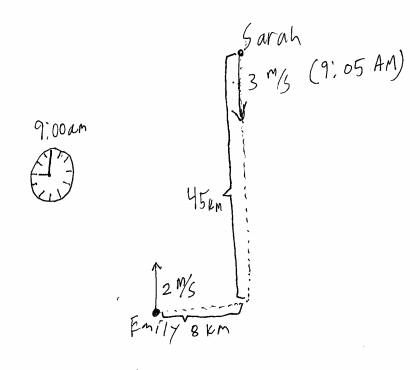
\includegraphics[scale=.75]{fig1}\caption{Our initial set-up for the problem}\label{setup}
\end{centering}\end{figure}

 Now, let's assign some coordinates to those points! I am going to declare that Emily's starting point is the origin, that is $(0,0)$. Then, this forces Sarah's starting point to be $(8000,45000)$ (all units are in meters here). Let's define a \emph{parametric} function $\vec{e}(t)$ giving Emily's position as a function of time (that is, $\vec{e}(t)$ should give us the coordinates of where she is at time $t$.) She's walking at 2 m/s, and if we declare time $t=0s$ to be 9:00am, then $\vec{e}(t)=(0,2t)$. Now we should do the same to find $\vec{s}(t)$, the function giving Sarah's position. There's a slight complication here though--technically Sarah's position should be given by a piecewise, because she stands still for the first five minutes. I'm going to choose to ignore that complication and instead model her path as if she starts walking at 9:00 am somewhere a bit north of her starting spot, so she passes through $(8000,45000)$ at $t=5$ min$=300$ s. This should give us the same answer if its the case that Sarah has started walking by the time they achieve their minimum distance--i.e. if the answer our method gives us is $\leq 300\st$, we should stop and rethink. That said, this gives $\vec{s}(t)=(8000, 45000-3(t-300))$ (be sure to think about why that gives us what we want)! Great, let's update our picture with all of this (Figure \ref{axes}).
 \begin{figure}[h!]\begin{centering}
 	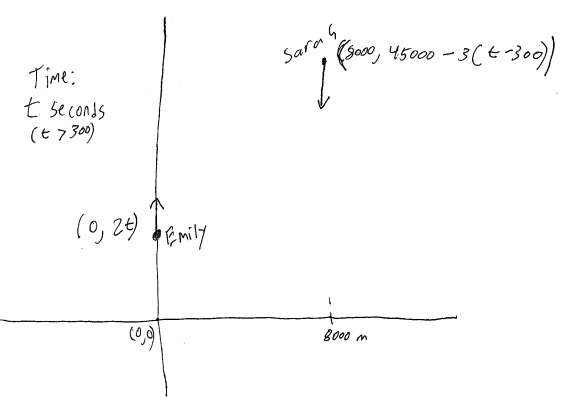
\includegraphics[scale=.7]{fig2}\caption{Our working picture now that we've given things coordinates and found position functions}\label{axes}
 \end{centering}\end{figure}
 Now, we want to model the distance between them. Let's name $\vec{e}(t)=(x_1,y_2)=(0,2t)$ and $\vec{s}(t)=(x_2,y_2)=(8000,45000-3(t-300))$. Call the distance between them $d(t)$ (Figure \ref{dist}).
 \begin{figure}[h!]\begin{centering}
 	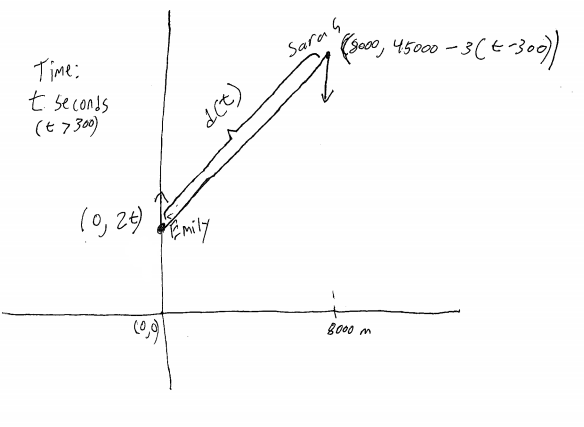
\includegraphics[scale=.7]{fig3}\caption{Our picture, now with the distance drawn in!}\label{dist}
 \end{centering}\end{figure}
 
  The distance formula (pythagorean theorem) gives \begin{align*}d(t)&=\sqrt{(x_1-x_2)^2+(y_1-y_2)^2}\\
 &=\sqrt{[0-8000]^2+[(2t)-(45000-3(t-300))]^2}\\
 &=\sqrt{(-8000)^2+(5 t-45900)^2}
 \end{align*}
Now, to find a minimum, we need to take a derivative of $d(t)$. This is messy but good practice\textemdash that said I'm going to skip going through all of that (it's just iterating the chain rule twice) and compute that $$d'(t)=\frac{5 t-45900}{\sqrt{t^2-18360 t+86832400}}$$
Now we just need to solve for when $d'(t)=0$! So long as our numerator and denominator aren't zero at the same time, this equates to setting the numerator equal to zero, giving $5t-45900=0$, or $t=9180\st=153\min=2\text{ hr, }33\min$. There's our answer!

So that's one way of doing it. However, Daniel Hall in my 9:00am section suggested a way of solving this problem which avoids doing any calculus altogether!\footnote{Sneaky, sneaky! This isn't a form of cheating, in fact it demonstrates excellent modeling/problem-solving intuition! This `ninja' solution didn't occur to me when I was writing the problem, and it's easy to miss stuff like this as a problem-writer. In essence, what I am saying is that if you need to solve a related rates problem, can't remember the calculus method but see some non-calculus way to do it, go for it! Your grader will be more impressed than anything else! That said, for now it's probably good practice to force yourself to solve things the calculus way. } He noticed that the (roads?) paths the two are walking are parallel, and the shortest line segment between two parallel lines is one which is perpendicular to them (Figure \ref{par}).

\begin{figure}[h!]\begin{centering}
	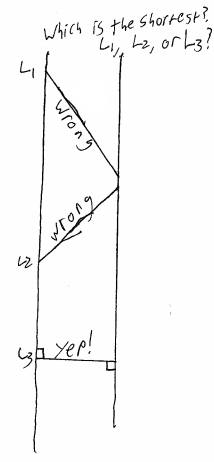
\includegraphics[scale=.6]{fig4}\caption{this was hard to draw correctly!}\label{par}
\end{centering}\end{figure}

 This observation tells us that since the horizontal distance never changes, all we need to do is determine when the vertical distance is zero. He modeled it such that $t=0$ at $9:05$, when Emily had already walked 600$\ml$ (that is, $(2\ms)(300\st)$). Now, the two girls start (vertically) $44,400\ml$ away from each other, so the equation we need to solve is $2t=44400-3t$, or $5t=44,400\implies t=8880\st=148$ min. Noticing that this corresponds to (9:05 AM+148 min)=11:33 AM=(9:00 AM+153 min) then gives the same answer we had before. 
\prob{3}
\textbf{Use linear approximation to estimate the following quantities (If you just plug each expression into a calculator I will be so, so deeply disappointed\textemdash unless you're just checking to see how close you are!):}

For this problem, what we have to do is \emph{(i)} identify some function $f$ so that the quantity we are trying to estimate can be viewed as $f(b)$ for some $b$, \emph{(ii)} find some $a$ nearby $b$ where it is easy to compute the \say{linear approximate,} that is, the tangent line, and \emph{(iii)} plug $b$ into the equation for that tangent line at $a$! Let's go through this process explicitly for each of these. 
\prt{1}
$$\sin(.005)\approx$$
\begin{enumerate}[label=\emph{(\roman*)}]
	\item $f(x)=\sin(x)$ seems like a natural choice, doesn't it? Then, $\sin(.005)=f(b)$ where $b=.005$
	\item $a=0$ is a nearby point that is easy to deal with! $f'(x)=\cos(x)$, so $f(a)=\sin(0)=0$ $f'(a)=\cos(0)=1$. Let's write out the formula for the tangent line at 0:
	$$L(x)=f'(a)(x-a)+f(a)=1*(x-0)+0=x$$
	\item  Plugging in $.005$ to $L$ gives $\sin(.005)\approx .005$.
\end{enumerate}
In reality, $\sin(.005)=.00499998\hdots$. As it turns out, our approximation was off only by $~2.08333\times 10^{-8}$, or on the order of one ten millionth!
\prt{2}$$e^{\ln(2)+.03}\approx$$
\begin{enumerate}[label=\emph{(\roman*)}]
	\item I would think that $f(x)=e^x$ is the only choice that is going to be that easy to deal with (note: we have a lot of freedom to make choices here, but some of those may be bad choices\textemdash not necessarily \emph{incorrect} choices, but \emph{bad}.) Then, $b=\ln 2+.03$.
	\item $a=\ln 2$ is going to be the easiest thing to deal with nearby for reasons we will see shortly. Then, $f(x)=e^x$ so $f'(x)=e^x$, and $f(a)=f'(a)=e^{\ln 2}=2$. Then, our tangent line will be given by $$L(x)=f'(a)(x-a)+f(a)=2*(x-\ln 2)+2$$
	\item Note $(b-a)=.03$ Then, $$L(b)=f'(a)(b-a)+f(a)=2(.03)+2=2.06$$ so $e^{\ln 2+.03}\approx 2.06$. 
	\end{enumerate}
In reality $e^{\ln 2+.03}=2.06091\hdots$, so our approximation was off by around $.00091$, or on the order of one thousandth.
\prt{3} $$(1000023)^{\frac{1}{6}}\approx$$
\begin{enumerate}[label=\emph{(\roman*)}]
	\item I think $f(x)=x^{1/6}$ is going to be a lot easier to deal with than $g(x)=(100023)^{x}$. Let's use $f$. Then, $b=1000023$
	\item Note that $x^{1/6}=\sqrt[6]{x}$. Thus, we should be looking around for sixth powers of things nearby. How about $10^6=1000000=b-23$? Sounds good to me, let's use $a=10^6$. Now, $f'(x)=\frac{1}{6}x^{-5/6}$. Plugging in $a$ gives $f'(a)=\frac{1}{6}(10^6)^{-5/6}=\frac{1}{6*10^5}=\frac{1}{600000}$.
	Of course $f(a)=(10^6)^{1/6}=10$. Then, $$L(x)=f'(a)(x-a)+f(a)=\frac{1}{6*10^5}(x-10^6)+10$$
	\item Notice $b-10^6=23$. Thus, $$L(b)=\frac{1}{6*10^5}(b-10^6)+10=\frac{1}{6*10^5}(23)+10=\frac{6000023}{600000}\approx10.00003833\hdots$$
	Gross!
\end{enumerate}
As it turns out, $(1000023)^{\frac{1}{6}}=10.00003833\hdots$\textemdash that's right, our approximation is so good that the error doesn't show up in the first ten decimal places! Using a computer algebra system (fancy calculator!), I computed that the actual error was around $3.67356*10^{-10}$ or on the order of one billionth! Amazing! Math!
\end{document}
